\section{Experiments}
\label{sec:experiments}

\begin{table*}[t]
  \centering\tabfont
  \caption{\textbf{Memory in reinforcement learning.}
  BSuite memory length~\cite{osband2020bsuite}: success as in R2I~\cite{samsami2024r2i}, \ie whether the evaluation return reaches 0.9 within the budget (\cmark) or not (\xmark); steps and returns in Supp.~\suppref{supp:impl}{A}. $^\dagger$Lengths, budget and training windows of R2I (1M steps; reward head with one output per action).
  POPGym RepeatPrevious~\cite{morad2023popgym} with the environment settings of R2I's code: max-mean episodic return, the metric of POPGym (chance $=-0.5$).
  \nr: not run, as the model fails at a shorter length.
  $^\ddagger$R2I with its official code and configuration for 2M steps, measured on its training episodes (for our models the two measures differ by at most 0.07).}
  \label{tab:rl}
  % generated by paper/scripts/paper_tables.py; do not edit
\begin{tabular}{@{}l cccc ccc cc@{}}
\toprule
 & \multicolumn{7}{c}{BSuite memory length: success} & \multicolumn{2}{c}{RepeatPrevious: return $\uparrow$} \\
\cmidrule(lr){2-8}\cmidrule(l){9-10}
 & $L$=8 & 16 & 32 & 64 & 51$^\dagger$ & 71$^\dagger$ & 101$^\dagger$ & Easy & Medium \\
\midrule
\swm~\cite{sun2025spikingwm} & \xmark & \xmark & \xmark & \xmark & \xmark & \xmark & \xmark & 0.64 & -0.46 \\
Recurrent LIF & \cmark & \xmark & \xmark & \xmark & \xmark & \nr & \nr & 0.74 & -0.44 \\
GRSN~\cite{qin2025grsn} & \cmark & \cmark & \xmark & \xmark & \xmark & \nr & \nr & 0.37 & -0.47 \\
DH-SNN~\cite{zheng2024dhsnn} & \cmark & \cmark & \xmark & \xmark & \xmark & \nr & \nr & -0.36 & -0.44 \\
TC-LIF~\cite{zhang2024tclif} & \cmark & \cmark & \cmark & \cmark & \cmark & \xmark & \cmark & 0.03 & -0.45 \\
\dv (ANN)~\cite{hafner2025dreamerv3} & \cmark & \cmark & \cmark & \xmark & \cmark & \xmark & \xmark & 0.42 & -0.41 \\
R2I (ANN)~\cite{samsami2024r2i} & \multicolumn{7}{c}{\footnotesize reported in~\cite{samsami2024r2i}, see text} & -0.48$^\ddagger$ & -0.46$^\ddagger$ \\
\midrule
\textbf{\method (ours)} & \cmark & \cmark & \cmark & \cmark & \cmark & \cmark & \cmark & 0.72 & 0.48 \\
\midrule
budget (env.\ steps) & 150k & 200k & 300k & 500k & 1M & 1M & 1M & 2M & 2M \\
\bottomrule
\end{tabular}

\end{table*}

\subsection{Setup}
\label{sec:setup}

\paragraph{Models.}
All models share one spiking world model, the network of \swm~\cite{sun2025spikingwm} built on DreamerV3 at the size of DreamerV3-S (512 units, $T=5$), and differ in the recurrent core:
\textbf{\swm} (multicompartment neurons with both resets, $\tau=2$);
\textbf{recurrent LIF} neurons, cleared at every environment step as usual in spiking RL;
\textbf{GRSN}~\cite{qin2025grsn}, gated recurrent spiking neurons;
\textbf{DH-SNN}~\cite{zheng2024dhsnn}, LIF neurons with eight dendritic branches of learned time constants;
\textbf{TC-LIF}~\cite{zhang2024tclif}, two-compartment LIF neurons for long sequences (GRSN, DH-SNN and TC-LIF update once per environment step and carry their state);
\textbf{\dv}~\cite{hafner2025dreamerv3}, the same architecture without spikes (GRU core, SiLU, one simulation step);
and \textbf{\method} with two PDN layers of $N=512$ neurons with $M=2$ channels, one integrator and one resonant.
R2I~\cite{samsami2024r2i}, a DreamerV3 agent with a state space recurrence and the state of the art among ANN world models on memory tasks, runs with its official code and configuration on POPGym; on BSuite we compare with its published results.
Within a benchmark, all models use identical hyperparameters, budgets and evaluation.
The actor and critic of every model read $(z_t,h_t)$; those of \method also read its dendritic state as spikes (\cref{sec:soma}), with 4.1M instead of 3.4M parameters (sizes in Supp.~\suppref{supp:impl}{A}, an actor-critic of 3.4M in Supp.~\suppref{supp:policy}{E}).

\paragraph{Benchmarks.}
We use benchmarks with published protocols and ANN results.
\textbf{BSuite memory length}~\cite{osband2020bsuite} shows a cue, then $L$ uninformative steps, and rewards the agent for recalling the cue; we run $L\in\{8,16,32,64\}$, and $L\in\{51,71,101\}$ with the lengths, budget (1M steps) and training windows of R2I~\cite{samsami2024r2i}.
\textbf{POPGym RepeatPrevious}~\cite{morad2023popgym} rewards the agent at every step for naming the suit of the card shown $k$ steps earlier ($k=4$ Easy, $k=32$ Medium), one of the three POPGym tasks with the highest memory demand that R2I evaluates; we use the environment settings of R2I's code for 2M steps.
\textbf{Memory Maze 9$\times$9}~\cite{pasukonis2023memorymaze} is first-person 3D navigation with episodes of 1000 steps; we use its offline probing benchmark with the official dataset and probes: after 1M world model updates with truncated backpropagation through time, probes decode the positions of the target objects (MSE) and the maze layout (accuracy) from the frozen state.
\textbf{DMC}~\cite{tassa2018dmc} walker walk from proprioception (500k steps, train ratio 512, as in DreamerV3) and from pixels (1M frames) serves as a control task without a memory demand; cheetah run and cartpole swingup from proprioception are in Supp.~\suppref{supp:impl}{A}.
On BSuite the reward depends on both the cue and the action, which the scalar reward head of a Dreamer world model does not learn within our budgets; all models therefore use a reward head with one output per action (Supp.~\suppref{supp:reward}{B}).
Supp.~\suppref{supp:impl}{A} gives the settings and the evaluation protocol of each benchmark.

\paragraph{World model probes.}
To measure memory without exploration and credit assignment, we also train world models alone on episodes of a random policy and measure the AUC of their reward prediction where the reward depends on the past, from 0.5 without memory to 1 with perfect recall: cue recall, BSuite memory length with the terminal reward set to the cue $L$ steps back ($\pm1$), and RepeatPrevious, where the reward indicates whether the action names the card $k$ steps back.
As in probing benchmarks~\cite{pasukonis2023memorymaze}, we report the final AUC after a fixed number of updates (Supp.~\suppref{supp:probe}{C}).

\subsection{Memory in reinforcement learning}
\label{sec:rl}

\begin{figure*}[t]
  \centering
  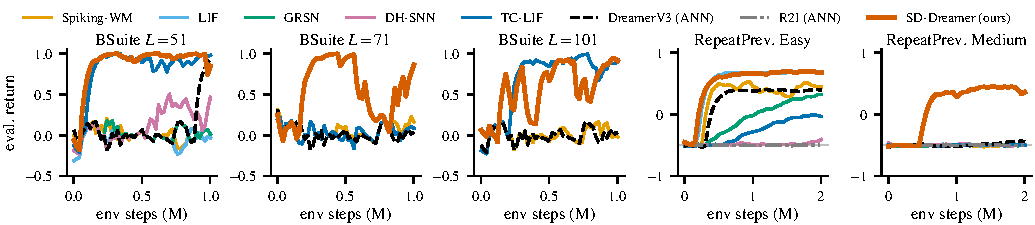
\includegraphics[width=\textwidth]{fig/rl_curves}
  \caption{\textbf{Learning curves} on BSuite memory length with the lengths and budget of R2I (left three) and POPGym RepeatPrevious (right two; chance $=-0.5$). Exponential moving average of the evaluation return (R2I: return of the training episodes, see \cref{tab:rl}).}
  \label{fig:rl_curves}
\end{figure*}

\Cref{tab:rl}, \cref{fig:memory_length} and \cref{fig:rl_curves} show how far each model remembers.
The spiking baselines remember as far as their neurons keep their state.
\swm, cleared at every step and at every spike, recalls no cue, not even 8 steps back, and recurrent LIF neurons, cleared at every step, solve 8 steps.
GRSN and DH-SNN carry leaky states across steps and solve 16 steps.
TC-LIF adds its input to two compartments that do not decay, and its spikes subtract a fixed amount from them instead of clearing them; it solves 64 steps and, with R2I's lengths, 51 and 101 steps, as the design rule of \cref{sec:amnesia} predicts; at 71 steps its return stays at 0.10.
\dv solves up to 32 steps in the short budgets and 51 steps with R2I's lengths (after 902k of 1M steps), and fails at 64, 71 and 101.

\method reaches a return of 0.9 at every length, as fast as the fastest baseline or faster: 64 steps after \numFwfToSixtyFour\ environment steps (TC-LIF 112k), and with R2I's lengths 51, 71 and 101 steps after \numFwfToFiftyOne, \numFwfToSeventyOne\ and \numFwfToHundredOne\ (TC-LIF 102k at 51 and 242k at 101 steps; returns in Supp.~\suppref{supp:impl}{A}).
R2I reports a median return of about 0.9 at 51 and 71 memory steps and about 0.35 at 101 after 1M steps (10 seeds; Fig.~7 of~\cite{samsami2024r2i}), with DreamerV3's default reward head and lengths that count one step less.

On RepeatPrevious Easy, \method reaches \numFwfEasy, close to the best baseline, recurrent LIF (0.74).
On Medium, which asks for the card of exactly 32 steps ago, every baseline, \dv included, stays at chance after 2M steps, while \method reaches \numFwfMedium.
R2I, run with its official code, stays at chance on both tasks within 2M steps.
In its published curves, R2I leaves chance on Medium only after about 3M steps, and DreamerV3 learns Easy but not Medium (Fig.~9 of~\cite{samsami2024r2i}), as in our runs.

\subsection{What the world model remembers}
\label{sec:probe}

\begin{table}[t]
  \centering\tabfont
  \caption{\textbf{World model probes} (data of a random policy, no policy). Final reward AUC (0.5 = no memory), mean of the last three evaluations after 12k (cue recall) or 10k (RepeatPrevious) updates; updates until 0.9 in Supp.~\suppref{supp:probe}{C}. $^\ast$Held out (used for no design choice): 20k updates, training window 128. \pend{Blue}: in progress.}
  \label{tab:probe}
  % generated by paper/scripts/paper_tables.py; do not edit
\setlength{\tabcolsep}{2.4pt}
\begin{tabular}{@{}l cccc ccc@{}}
\toprule
 & \multicolumn{4}{c}{cue recall} & \multicolumn{3}{c}{RepeatPrevious} \\
\cmidrule(lr){2-5}\cmidrule(l){6-8}
 & $L$=8 & 16 & 32 & 64 & $k$=4 & 32 & 64$^\ast$ \\
\midrule
\swm~\cite{sun2025spikingwm} & 0.49 & 0.54 & 0.66 & 0.52 & 0.97 & 0.50 & 0.50 \\
Recurrent LIF & 1.00 & 0.52 & 0.50 & 0.50 & 0.99 & 0.50 & 0.50 \\
GRSN~\cite{qin2025grsn} & 1.00 & 1.00 & 0.51 & 0.51 & 0.89 & 0.51 & 0.50 \\
DH-SNN~\cite{zheng2024dhsnn} & 1.00 & 1.00 & 1.00 & 0.52 & 0.63 & 0.50 & \pend{0.50} \\
TC-LIF~\cite{zhang2024tclif} & 1.00 & 1.00 & 1.00 & 1.00 & 0.86 & 0.50 & 0.57 \\
\dv (ANN)~\cite{hafner2025dreamerv3} & 1.00 & 1.00 & 1.00 & 0.50 & 0.95 & 0.50 & 0.50 \\
\midrule
\textbf{\method (ours)} & 1.00 & 1.00 & 1.00 & 1.00 & 0.98 & 0.92 & 0.94 \\
\bottomrule
\end{tabular}

\end{table}

The probes separate memory from policy learning (\cref{tab:probe}).
On cue recall, \method and TC-LIF recall 64 steps (AUC 1.00); DH-SNN and \dv stop at 32, GRSN at 16, recurrent LIF at 8, and \swm recalls no length.
The order is that of RL, so the limits of the baselines are limits of their world models.

RepeatPrevious asks for a different memory: the input of an exact lag among a stream of similar inputs.
At $k=4$ most models learn it (AUC 0.86 to 0.99; \method 0.98).
At $k=32$, \method is the only model that learns it (AUC 0.92); all others, TC-LIF and \dv included, stay at 0.50 to 0.51.
Resonance is the reason: without resonant channels the same model reaches only 0.57 (\cref{tab:ablation}).
TC-LIF recalls the cue 64 steps back as well as \method, but its compartments oscillate without decay at one period of about 12 steps that all neurons share (Supp.~\suppref{supp:impl}{A}), whereas each resonant channel of \method has its own phase and retention time.
We added resonant channels after an earlier model with integrator channels only failed this task (Supp.~\suppref{supp:diag}{F}) and used RepeatPrevious Hard ($k=64$) for no design choice.
On Hard, \method reaches an AUC of 0.94, and all other models stay at 0.50 to 0.57.

\begin{figure*}[t]
  \centering
  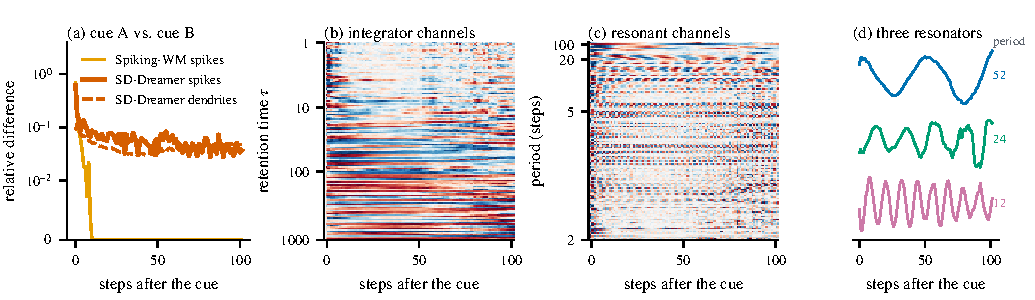
\includegraphics[width=\textwidth]{fig/dendrites_viz}
  \caption{\textbf{Where the cue is held} (BSuite memory length 101, world models of the agents of \cref{tab:rl}). Two evaluation episodes that differ only in the cue enter each world model, with the stochastic state at its mode, so that the two runs differ only through the cue.
  (a) Difference between the two episodes, relative to the mean, of the spikes that carry the recurrent state to the next step (\swm: its recurrent core; \method: the second PDN layer) and of the dendritic channels of \method.
  (b, c) Difference of each channel of the second PDN layer, scaled to the largest value of the channel: integrator channels sorted by retention time, resonant channels by period $2\pi/\theta$.
  (d) Three resonant channels with retention times above 200 steps; numbers: period in steps.}
  \label{fig:dendrites}
\end{figure*}

\Cref{fig:dendrites} shows where this memory lives, in the world models of the agents on BSuite memory length 101.
When two episodes differ only in the cue, the spikes of \swm become identical 10 steps after the cue, since no state outlasts the step reset.
In \method, the dendritic channels keep the difference for all 101 steps, and so do the spikes of the soma (3\% of the firing rate at the query).
Integrator channels with long retention times hold the difference with a constant sign, and each resonant channel rotates it with its own period, so that its phase encodes the time since the cue.

\subsection{Memory Maze}
\label{sec:mm}

\begin{table}[t]
  \centering\tabfont
  \setlength{\tabcolsep}{3pt}
  \caption{\textbf{Memory Maze and DMC walker walk.} Memory Maze 9$\times$9 offline probing~\cite{pasukonis2023memorymaze}: probes on the frozen state after 1M updates, second half of the evaluation episodes (constant predictor: 23.9 MSE, 80.8\% walls). Walker walk: return after 500k steps from proprioception and after 1M frames from pixels. \nr: not run. Bottom: reference results from~\cite{pasukonis2023memorymaze} (larger RSSM).}
  \label{tab:mm}
  % generated by paper/scripts/paper_tables.py; do not edit
\begin{tabular}{@{}l cc ccc@{}}
\toprule
 & \multicolumn{2}{c}{Memory Maze 9$\times$9} & \multicolumn{3}{c}{DMC return $\uparrow$} \\
\cmidrule(lr){2-3}\cmidrule(l){4-6}
 & obj.\ MSE $\downarrow$ & walls \% $\uparrow$ & walk & run & swing \\
\midrule
\swm~\cite{sun2025spikingwm} & \pend{11.9} & \pend{83.1} & 923 & 343 & 497 \\
Recurrent LIF & \pend{11.8} & \pend{83.6} & \pend{906} & \pend{263} & \pend{390} \\
GRSN~\cite{qin2025grsn} & \pend{11.6} & \pend{83.1} & \pend{594} & \pend{146} & \pend{447} \\
\swmnr & \pend{11.2} & \pend{83.4} & \pend{659} & \pend{180} & \pend{203} \\
\dv (ANN)~\cite{hafner2025dreamerv3} & 9.8 & 85.3 & 953 & 699 & 871 \\
\midrule
\textbf{\method (ours)} & \pend{9.2} & \pend{82.9} & 908 & \pend{382} & \pend{481} \\
\midrule
RSSM~\cite{pasukonis2023memorymaze} & 8.3 & 89.0 & \nr & \nr & \nr \\
RSSM, TBTT~\cite{pasukonis2023memorymaze} & 6.2 & 94.0 & \nr & \nr & \nr \\
\bottomrule
\end{tabular}

\end{table}

Memory Maze tests whether a world model builds a map of a 3D maze from first-person views over 1000 steps.
\Cref{tab:mm} reports the probes on the state that the policy reads: $(z_t,h_t)$ for all models, and in addition the dendritic spikes for \method.
\method locates the target objects more accurately than \dv (MSE 9.0 against 9.8) and every spiking baseline (11.5 to 12.6).
On the wall layout, all models of this size stay within 5 points of the constant predictor (80.8\%), \method at 83.7\% and \dv at 85.3\%; the larger RSSM of~\cite{pasukonis2023memorymaze} reaches 89.0\%.
\Cref{fig:mm_viz} shows what this memory does.
While an object is in view, every model locates it (squared error 1.4 to 3.5).
Once the object leaves the view, the error of the spiking baselines rises within 3 to 5 steps to 7.3 to 11.7, whereas \method stays at \pend{3.8} and has the lowest error of all models, \dv included, from 6 to 100 steps after the object left the view.
\TODO{Memory Maze: final probes after 1M updates (in progress); the values are the latest probes during training.}

\begin{figure*}[t]
  \centering
  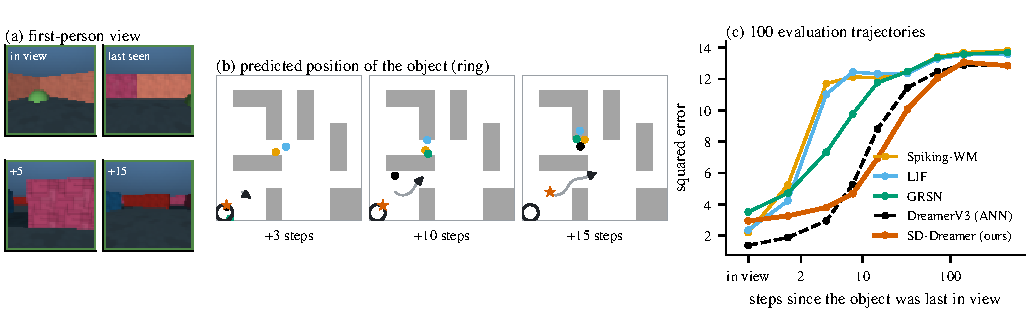
\includegraphics[width=\textwidth]{fig/mmaze_viz}
  \caption{\textbf{Memory of objects out of view} (Memory Maze 9$\times$9, the probes of \cref{tab:mm}).
  (a) First-person views around the first time, in evaluation trajectory 0, that an object in view for 5 steps leaves the view for at least 40 steps.
  (b) The position of this object (ring) that the probe of each model predicts 3, 10 and 15 steps later (\method: star); arrow: the agent; grey: its path since it last saw the object.
  (c) Squared error of the predicted object position against the steps since the object was last in view (within the $90^\circ$ field of view, no wall in between), first 100 evaluation trajectories.
  \pend{\method: checkpoint after 330k of 1M updates.}}
  \label{fig:mm_viz}
\end{figure*}

\subsection{Causes of reset amnesia}
\label{sec:causal}

\begin{table}[t]
  \centering\tabfont
  \caption{\textbf{Interventions on \swm} (world model probe, cue recall over $L$ steps). Updates until the reward AUC exceeds 0.9, two seeds; -- = not within 12k updates; blank = not run. A: state kept across environment steps; B: no dendritic reset on a somatic spike; G: dendritic input scaled by $\sqrt{\tau_d/2}$. GRU: reference core with continuous state.}
  \label{tab:interventions}
  % Phase 0 (PHASE0.md §4.1): seeds s0 / s1, updates until reward AUC > 0.9 (k = thousand updates)
\begin{tabular}{@{}lcccc ccc@{}}
\toprule
 & A & B & G & $\tau_d$ & $L=8$ & $L=16$ & $L=32$ \\
\midrule
\multirow{3}{*}{\swm} & & & & 2 & -- / -- & -- / -- & 12k / -- \\
 & & & & 16 & -- / -- & -- / -- & \\
 & & & & 128 & -- / -- & -- / -- & \\
\midrule
B only & & \cmark & & 128 & -- / -- & & \\
G only & & & \cmark & 128 & & -- / -- & \\
\multirow{2}{*}{A} & \cmark & & & 2 & -- / 9k & -- / -- & \\
 & \cmark & & & 128 & 3k / 4k & 8k / 8.5k & \\
A+B & \cmark & \cmark & & 128 & 3k / 3k & 4.5k / 4.5k & -- / -- \\
A+B+G & \cmark & \cmark & \cmark & 128 & \textbf{0.5k / 0.5k} & \textbf{0.5k / 0.5k} & \textbf{2k / 3k} \\
\midrule
GRU core & \multicolumn{4}{c}{continuous state} & 0.5k / 0.5k & 1k / 1k & 5k / 3.5k \\
\bottomrule
\end{tabular}

\end{table}

We test the three mechanisms of \cref{sec:amnesia} with interventions on \swm in the cue recall probe (\cref{tab:interventions}; details in Supp.~\suppref{supp:probe}{C}).
\textbf{A} keeps all compartments across environment steps and clears them only at episode starts, \textbf{B} keeps the dendrites when the soma fires, and \textbf{G} multiplies the dendritic input by $\sqrt{\tau_d/2}$, which equalizes the stationary spread across dendritic time constants $\tau_d$.

\textbf{With resets, time constants do not matter.}
\swm fails at 8 and 16 steps for $\tau_d\in\{2,16,128\}$, and the cue can be decoded from its spikes for only 2 to 3 steps after it is shown.
At 32 steps, one of two seeds crosses an AUC of 0.9 at the last of 12k updates by holding the cue in self-sustained recurrent firing, a memory that exists only as spikes.
\textbf{Persistence is necessary.}
Without A, neither B nor G helps.
With A and $\tau_d=128$, the world model recalls 8 and 16 steps; removing the dendritic reset too (A+B) nearly halves the updates at 16 steps (4.5k instead of 8k to 8.5k).
\textbf{The write gain limits long time constants.}
With both resets removed, a cue moves the basal potential of a $\tau_d=128$ dendrite by 0.004 to 0.009, about 1\% of the threshold, against 0.19 at $\tau_d=2$.
A+B therefore fails at 32 steps, although a linear probe still decodes the cue from the membrane potentials at the recall step (accuracy 0.88): the trace is there, but too faint to drive spikes.
Restoring the gain (A+B+G) recalls 8 and 16 steps within 500 updates and 32 steps within 2000 to 3000, faster than the GRU core, and still learns 32 steps in 2000 updates with the firing rate capped at 0.06.
\textbf{Longer memory needs more than removing resets.}
A+B+G fails at 64 steps even with $\tau_d=512$, and in reinforcement learning it stops at 32 steps (\swmnr in Supp.~\suppref{supp:impl}{A}).
Its time constants are counted in simulation steps, and its soma still resets; a PDN counts retention times in environment steps and has a stateless soma.

\subsection{Ablations}
\label{sec:ablation}

\begin{table}[t]
  \centering\tabfont
  \caption{\textbf{Ablations} on the world model probes (as in \cref{tab:probe}). Each row changes one design choice of \method.}
  \label{tab:ablation}
  % generated by paper/scripts/paper_tables.py; do not edit
\begin{tabular}{@{}l cc c c@{}}
\toprule
 & \multicolumn{2}{c}{cue recall} & RepeatPrev. & firing \\
\cmidrule(lr){2-3}
variant & $L$=32 & 64 & $k$=32 & rate \\
\midrule
\method & 1.00 & 1.00 & 0.92 & 0.25 \\
\midrule
dendrites cleared every step & 0.51 & 0.50 & 0.50 & 0.25 \\
single $\tau=16$ & 1.00 & 0.49 & 0.92 & 0.24 \\
single $\tau=128$ & 1.00 & 1.00 & 0.93 & 0.26 \\
$\tau$ fixed at initialization & 1.00 & 1.00 & 0.93 & 0.24 \\
Euler write gain $1-\lambda$ & 1.00 & 0.52 & 0.76 & 0.21 \\
one PDN layer & 1.00 & 0.50 & 0.91 & 0.21 \\
one PDN layer, $T=1$ & 0.99 & 0.99 & 0.50 & 0.15 \\
no resonant channels & 1.00 & 1.00 & 0.57 & 0.27 \\
all channels resonant & 1.00 & 1.00 & 0.95 & 0.23 \\
firing rate capped at 0.06 & 1.00 & 0.51 & 0.92 & 0.06 \\
soma with membrane and reset & 1.00 & 0.52 & 0.77 & 0.18 \\
Heaviside soma & 1.00 & 1.00 & 0.88 & 0.16 \\
$M=4$ channels & 1.00 & 1.00 & 0.93 & 0.25 \\
no spike feedback & 1.00 & 1.00 & 0.94 & 0.23 \\
\bottomrule
\end{tabular}

\end{table}

\Cref{tab:ablation} changes one design choice at a time (updates until 0.9 in Supp.~\suppref{supp:probe}{C}).
\textbf{PDM}: clearing the dendrites at every environment step erases the memory (AUC 0.50 to 0.51 on all three tasks), the direct test of reset amnesia inside our own model.
\textbf{Retention time}: a single retention time of 16 steps fails at 64 steps and one of 128 succeeds; the spectrum from 1 to 1000 steps succeeds without being set for the task, learned or kept at its initialization.
\textbf{NWG}: with the Euler gain $1-\lambda$ the channels with long retention times are too faint, and the model fails at 64 steps (0.52) and reaches only 0.76 at $k=32$.
\textbf{Stateless soma}: a soma that keeps a membrane potential and is reset by its spike fails at 64 steps (0.52) and reaches 0.77 at $k=32$.
\textbf{Resonance}: without resonant channels the model fails at $k=32$ (0.57); with resonant channels only it solves all three tasks, as does \method with one channel of each kind.
\textbf{Depth and sparsity}: one PDN layer, or a firing rate capped at 0.06 (from 0.25), fails at 64 steps.
The spike count, the feedback and the number of channels leave the memory nearly unchanged (AUC 0.88 to 0.94 at $k=32$); the spike count and the feedback serve the prediction of motion: on the same pixel walker episodes, the world model with both predicts the next frame as well as recurrent LIF neurons (image loss 44.3 vs.\ 44.1), and with one spike per step it does not (55.3; Supp.~\suppref{supp:diag}{F}).

\subsection{Control tasks}
\label{sec:control}

On walker walk from proprioception (\cref{tab:mm}), \method reaches \numFwfDmcWalk, the highest return of the spiking models together with \swm.
From pixels (\numFwfPixWalk) and on cheetah run and cartpole swingup from proprioception (Supp.~\suppref{supp:impl}{A}), it ranks second among the spiking baselines, after recurrent LIF.
From pixels, every world model predicts the walker from the actions alone for about 10 to 20 steps (\cref{fig:walker_viz}); the frames that \method predicts stay closer to the observed ones than those of \swm at all 45 steps, and than those of \dv from step 15 on.

\begin{figure*}[t]
  \centering
  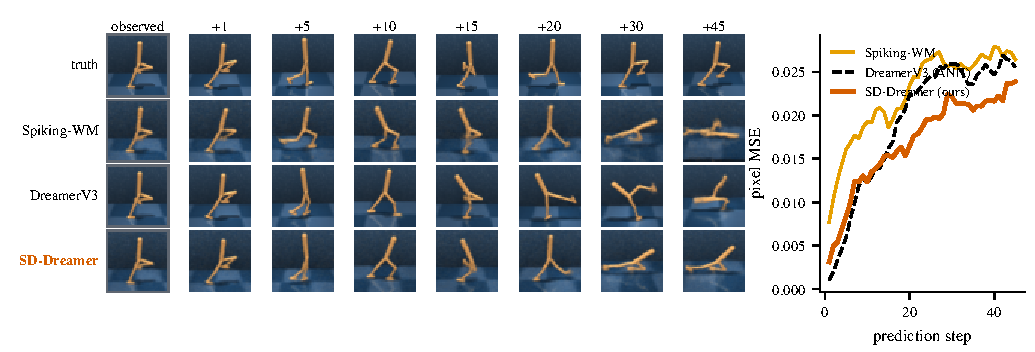
\includegraphics[width=\textwidth]{fig/walker_viz}
  \caption{\textbf{Open-loop prediction from pixels} (DMC walker walk). Each world model observes 5 frames of the same evaluation episode of \method and then predicts 45 frames from the actions alone.
  Right: pixel MSE of the predicted frames, mean over 8 segments of the episode.
  \pend{\method: checkpoint after 448k of 1M frames.}}
  \label{fig:walker_viz}
\end{figure*}

